\chapter[Grafana]{Grafana \\
\small{\textit{-- JGa, JGr, CS}}
\index{Grafana} 
\index{Chapter!Grafana}
\label{Chapter::Grafana}}

In this chapter, we discuss the setup of Prometheus, Node Explorer, and Grafana. Prometheus is a tool that monitors and collects metrics from various targets.
Node Exporter exposes detailed operating system metrics on the host including CPU, memory, disk, and network usage.
Prometheus scrapes these metrics from Node Exporter and stores them for analysis and visualization in Grafana. 

\begin{figure}[h]
  \centering
  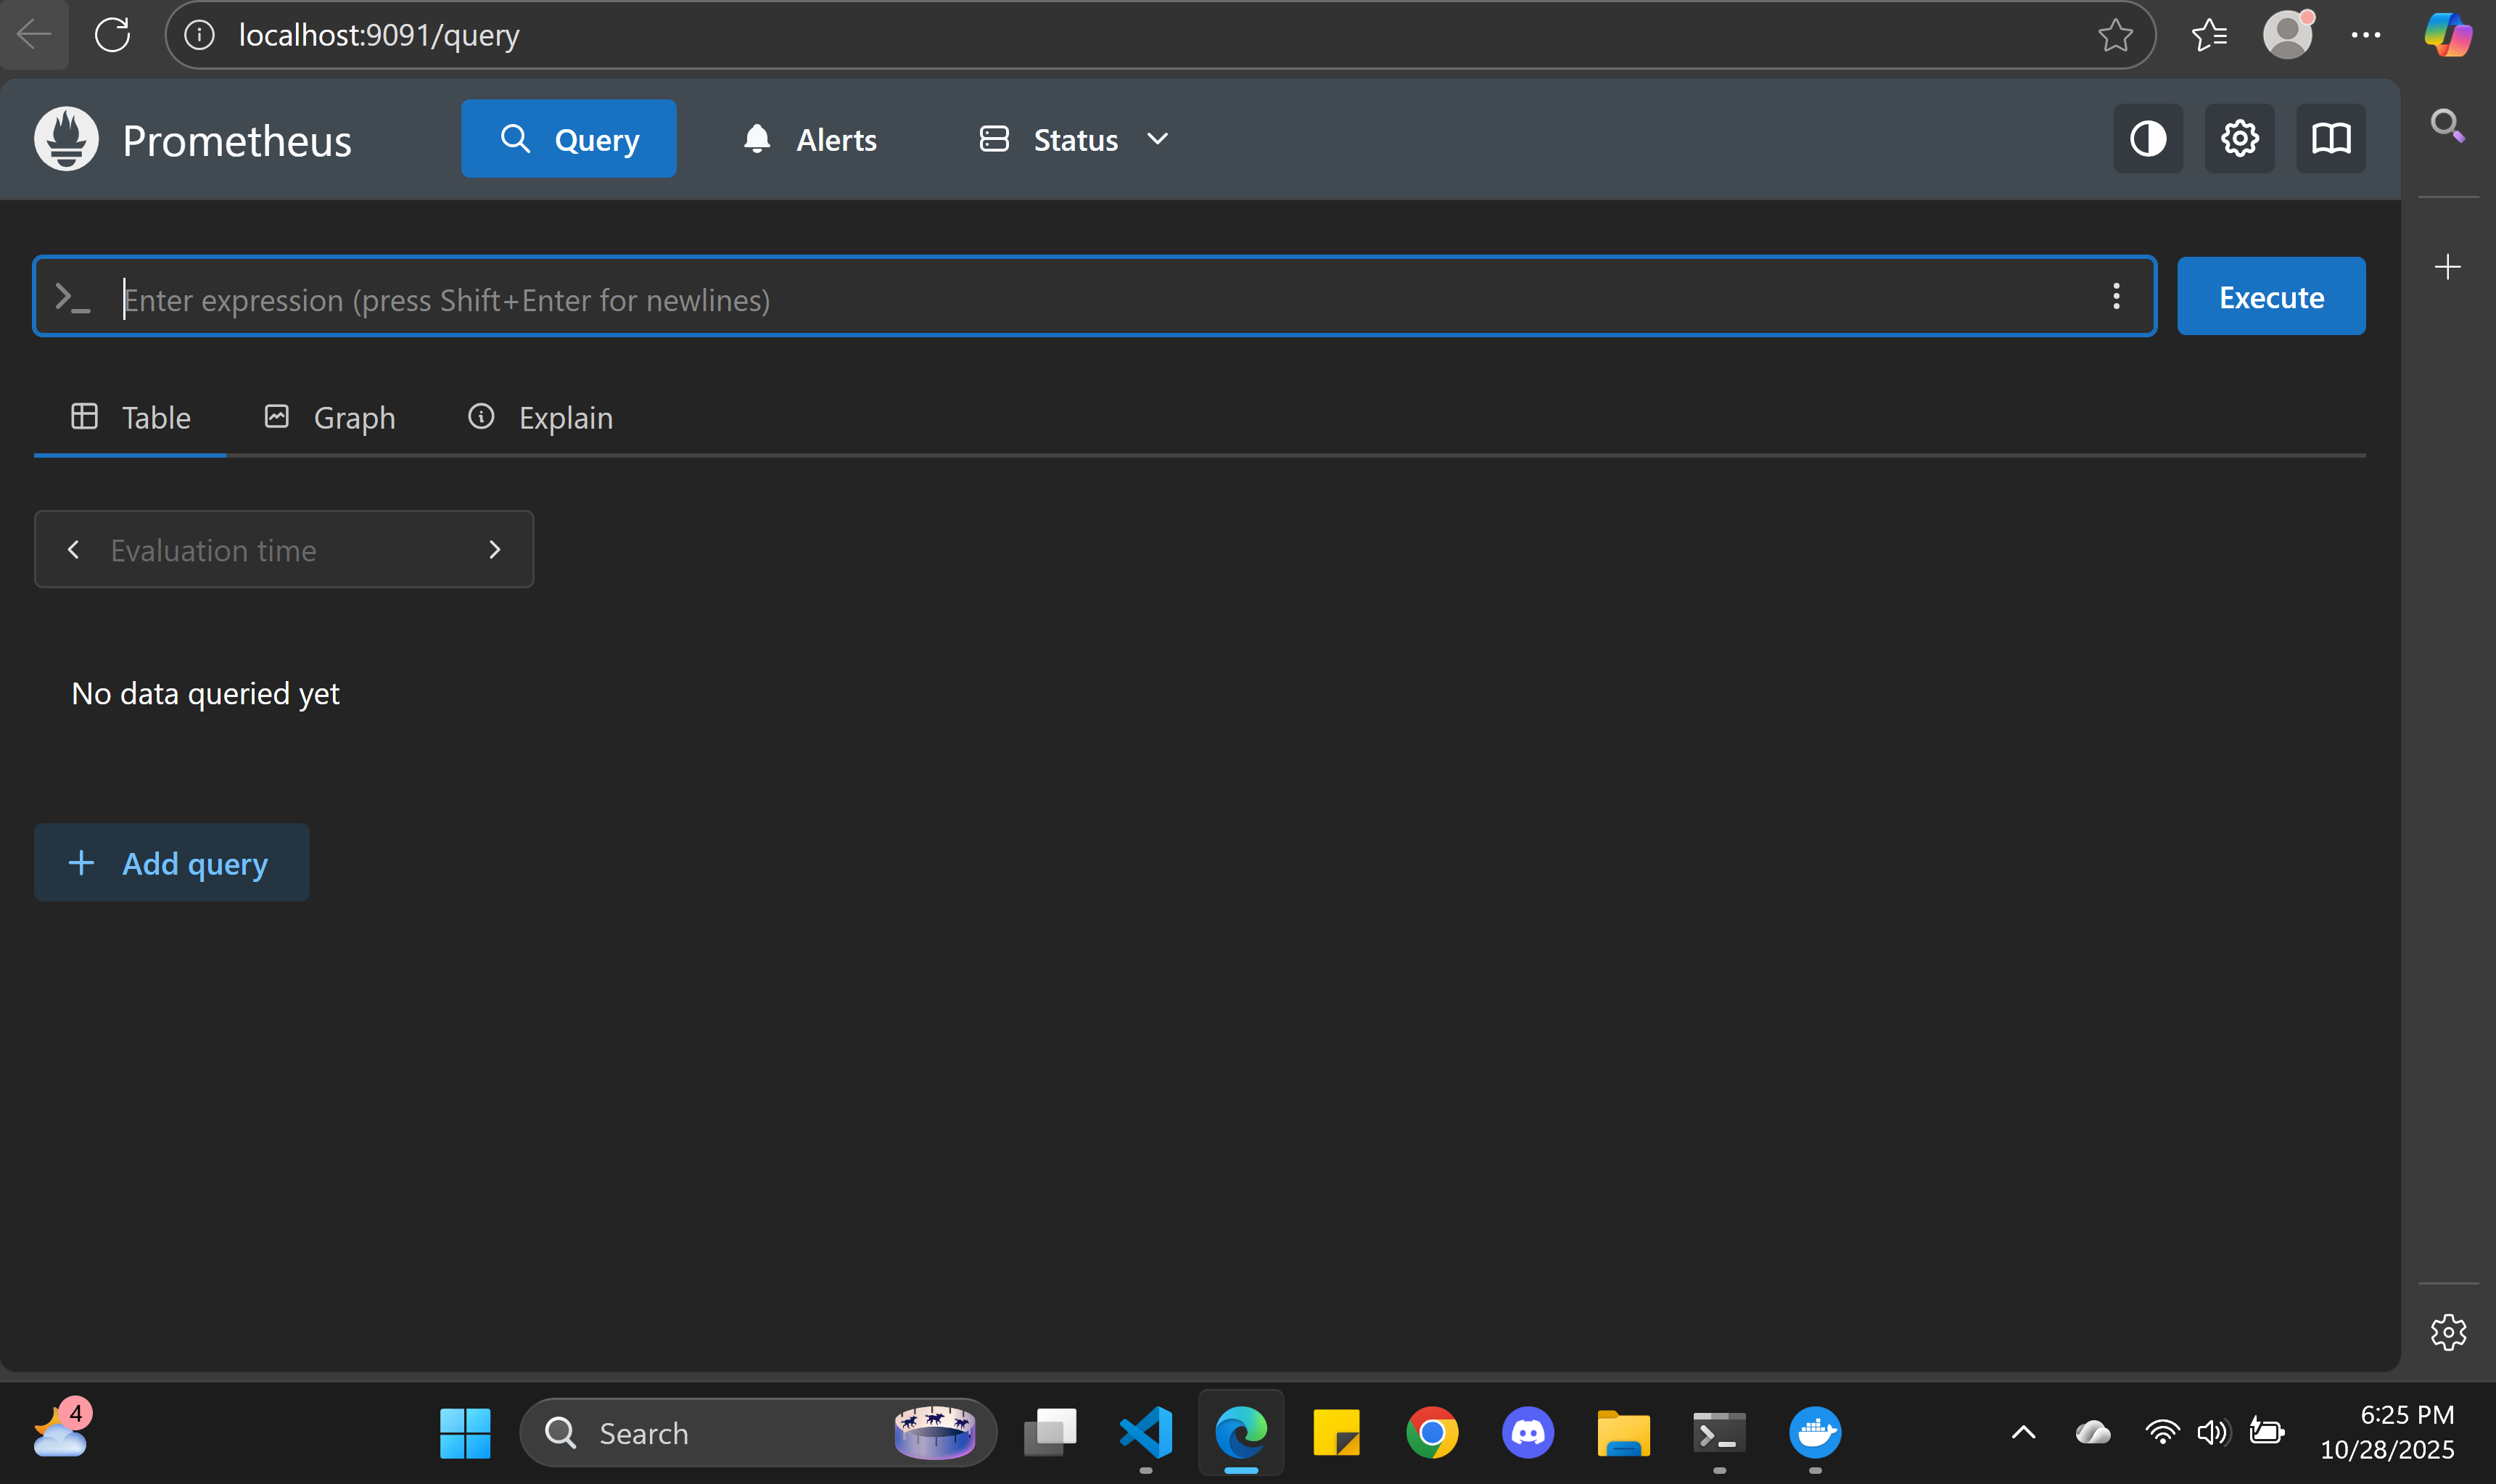
\includegraphics[width=0.7\textwidth]{png/prometheus_ss.png}
  \caption{Prometheus running through Docker on http://localhost:9091.}
  \label{fig:prometheus_ss}
\end{figure}

Grafana provides dashboards that sync to the Prometheus data source, which can be refreshed at specified intervals, 
allowing for easy viewing of the host's real-time system performance metrics.
The Grafana Dashboard 1860, the “Node Exporter Full” dashboard, visualizes key indicators of system health, 
including CPU load, memory utilization, RAM usage, and disk I/O activity.
Together, these tools create a stack that enables easy monitoring and diagnosis of performance issues on the host system, as seen in Figure 10.2.

\begin{figure}[h]
  \centering
  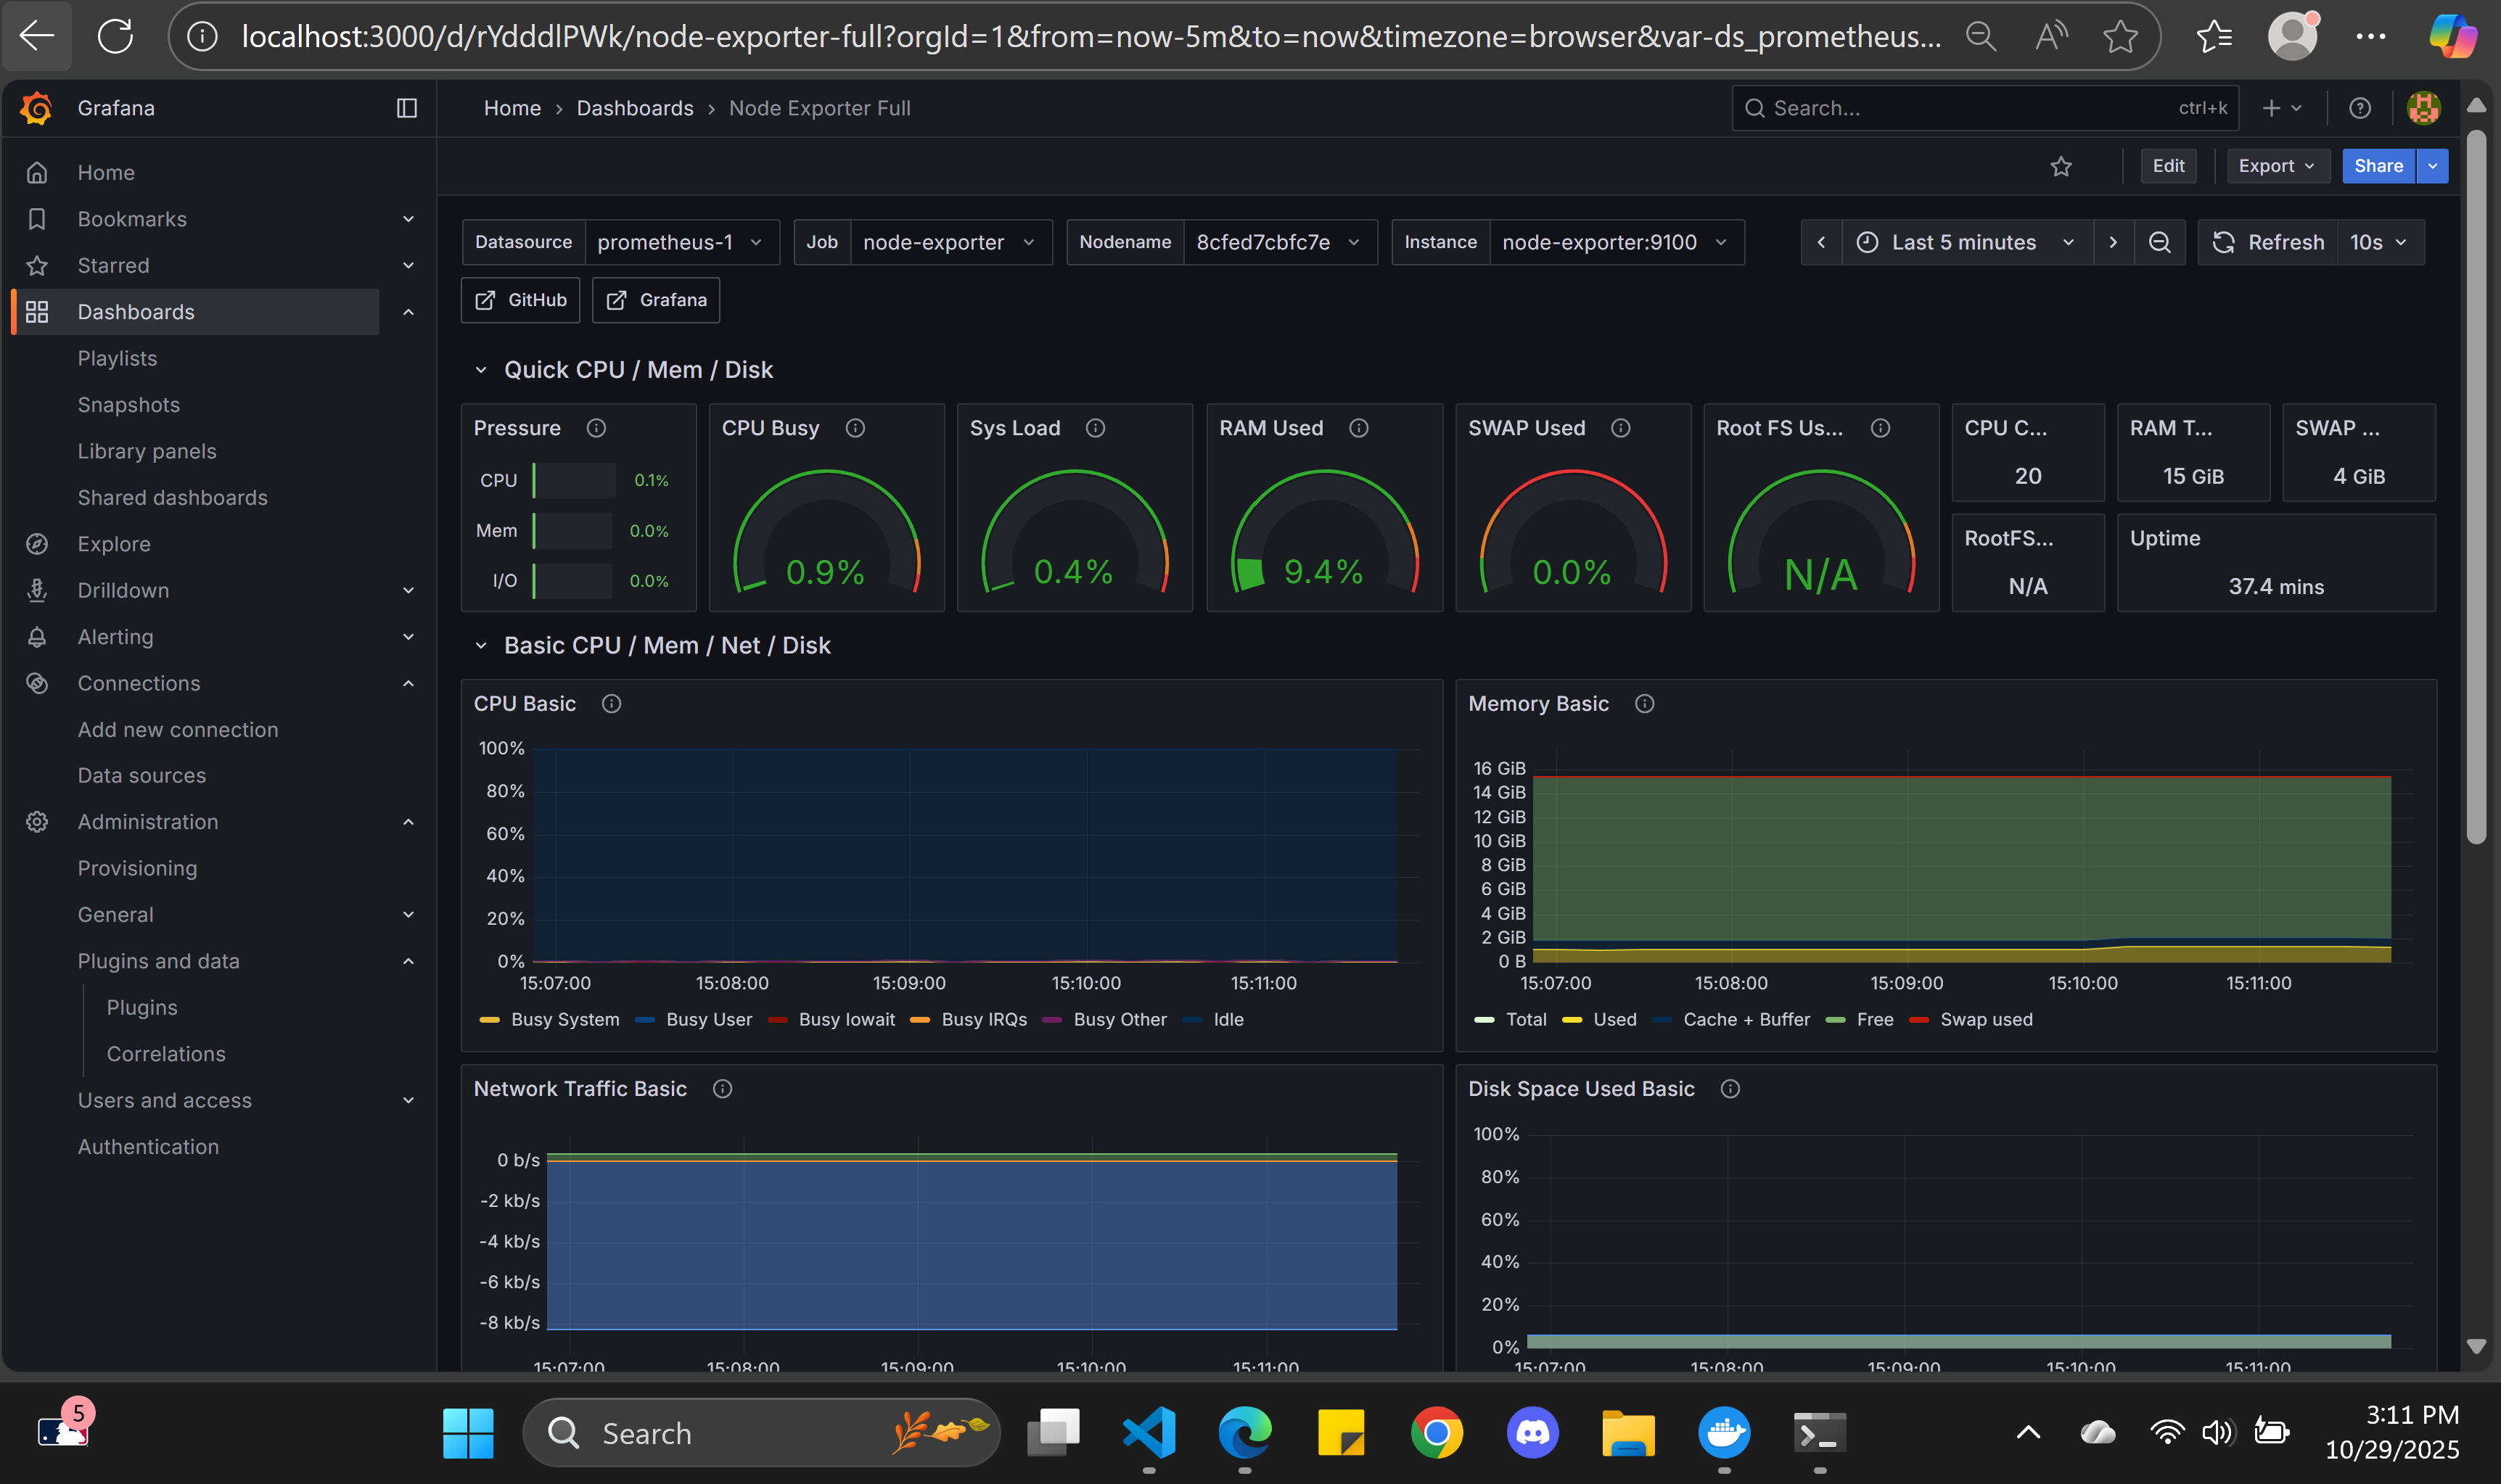
\includegraphics[width=0.7\textwidth]{png/grafana_dash1860_ss.png}
  \caption{Live Grafana dashboard 1860 with local host performance metrics displayed.}
  \label{fig:grafana_dash1860_ss}
\end{figure}
